\chapter{Read Error Correction}
\label{chap:read-error-correction}

Read data used as an input to many assembly algorithms contain plenty of errors, such as wrongly read bases. The make the data usable for assembly, an error correction step is required. Howerver, it does not remove all the errors and assembly algorithms must work cope with that fact, especially when dealin gwith read ends.

Currently, two different approaches are used to correct read errors, and both are based on transforming individual reads into series of k-mers. One is based on detecting errors as low covered edges (or paths) in a De Bruin graph, the another relies on a k-mer frequence distribution. During development of our algorithm covered in this thesis, we made several attempts to implement an error correction algorithm based on De Bruin graphs. Since we use these graphs also during assembly performing error corrections on them seemed to be a natural choice. Although they definitely imrpoved quality of the input reads, all our attempts did not produce results as good as solutions based on k-mer frequency distribution.

In the end, we decided to adopt the error correction algorithm used by the \texttt{fermi-lite} application and based on k-mer frequency disbribution. This chapter covers the algorithm in great detail, although it also gives basic information related to usage of De Bruin graphs.

\section{De Bruin Graphs}
\label{sec:ec-de-bruin-graphs}

This method involves transforming the input reads into a De Bruin graph in a way very similar to one used by our assembly algorithm. Although implementation details may differ, the basic idea is the same: each read mapped to certain active region is divided into a sequence of k-mers, each k-mer serves as a vertex and the edges follow the k-mer order within the sequence. Reference sequence, covering the active region, may also be included in the graph.

The most important assumption is that errors produce unique, and thus with low read coverage, connection between graph vertices. Low-covered edges with source vertices with output degree greater than one are especially interesting. Even a change of a single base in read sequence may divert the path representing the read through edges with higher read coverage. The locality of the change depends on used k-mer size.

A simple example demonstrating the main idea is displayed on Figure \ref{fig:error-correction-db}. Many reads share a sequence of \texttt{TTGCGCTAA}. Howerver, there is also a single read that contains a sligtly different sequence of \texttt{TTGCACTAA}. The De Bruin graph shown on the left part of the figure uses k-mers 4 bases long, and combination of both sequences produces a standard bubble.

If the bubble was supported by reasonable amount of reads, it would be trated as a SNP. Since only one read supports it, it may be reasonable to consider its divergence from other reads as an error, and to correct it, so the read path would follow more populated edges. When the correction is done, the resulting graph becomes linear, as the right part of Figure \ref{fig:error-correction-db} shows.

\begin{figure}[h]
	\centering
	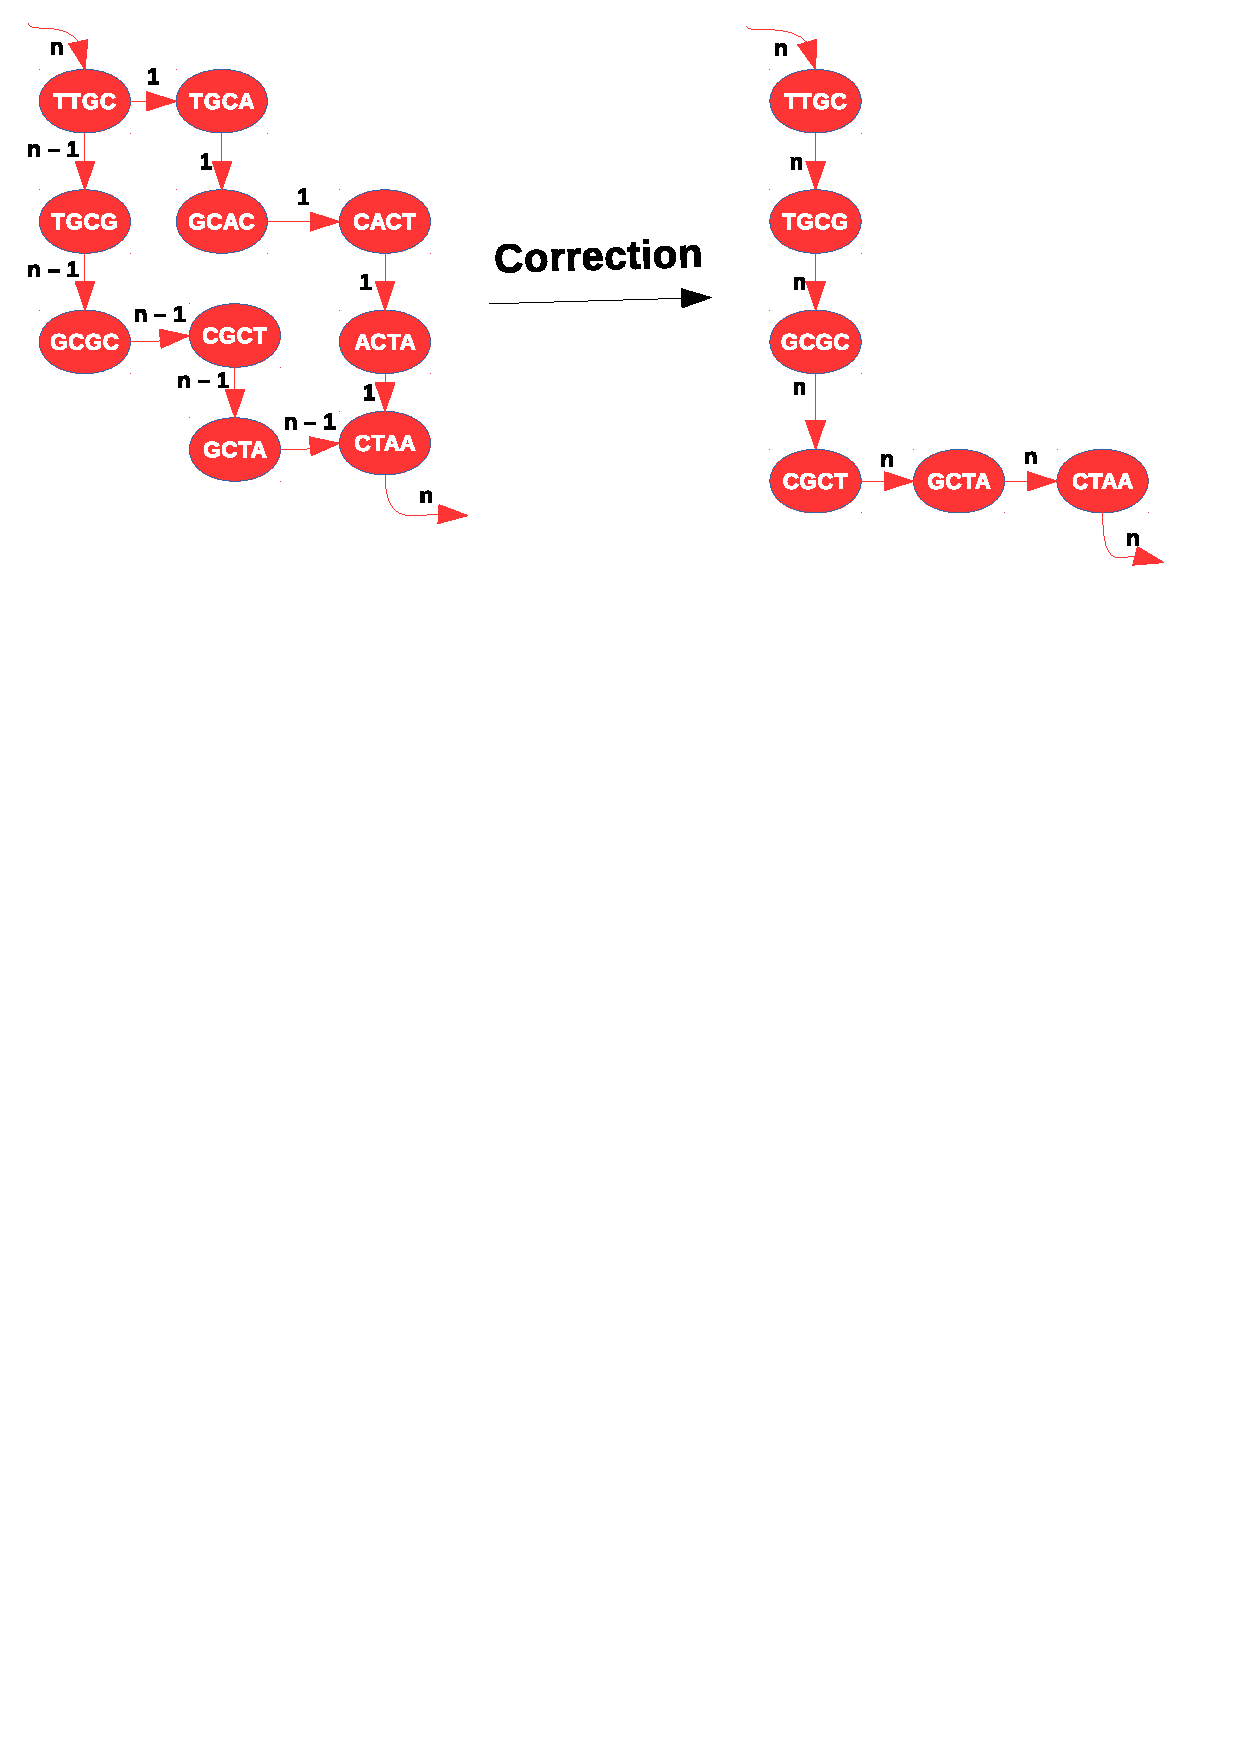
\includegraphics{img/error-correction-db.pdf}
	\caption{Simple examle of a read error detection by utilizing De Bruing graphs}
	\label{fig:error-correction-db}
\end{figure}

\section{K-mer Frequency Distribution}
\label{sec:ec-kmer-frequency-distribution}

